\chapter{MegaManaging, Part II: Direction, Growth, and the Design of an Extraordinary Life}

We begin with arithmetic, but the arithmetic is only bait. In this Jim Rohn seminar talk, preserved through a curated LazyingArt LLC playlist and reconstructed through Video2Book, a sales-management audience is led from a simple ladder of earnings to a much larger claim: what changes a life is not first the market, but the person brought to the market. The lecture then widens from this numerical opening into a geometry of direction, a drama of opposites, a redesign of the five-year future, and finally a discipline of work, measurement, and lifestyle.

\section{The Income Ladder and the Marketplace of Value}

Rohn opens by asking a question which is numerical in form and philosophical in consequence: is it possible to multiply income by \(10\)? He does not begin with abstraction. He begins with observed cases. If someone in the local market earns \(\$50\) an hour, then the first multiplication is already on the table. If someone earns \(\$500\) an hour, the second multiplication is already on the table. If well-known figures can command very large speaking fees, then the ladder is not imaginary; it is already populated.

The opening arithmetic can be written in the compact form
\begin{align}
50 \times 10 &= 500,\\
500 \times 10 &= 5000.
\end{align}
If we let \(I_n\) denote the earning level at the \(n\)-th rung of the ladder, then the lecture is using the recurrence
\begin{equation}
I_{n+1}=10I_n.
\end{equation}

\begin{remark}
This recurrence is a note-writer's shorthand. It is faithful to the arithmetic of the lecture, but it is not spoken as an algebraic formula.
\end{remark}

Rohn then blocks the natural objection that the ladder is too extreme by adding concrete scale points: roughly \(\$65{,}000\) for a one-hour speech, roughly \(\$125{,}000\) for a one-hour speech, and an annual figure of \(\$36\) million for a year's work. The purpose is not celebrity worship. The purpose is to make the possibility claim difficult to dismiss.

But the lecture does not stay with money for long. The real pivot comes with the phrase ``as high as you wish,'' followed immediately by the correction that what is really at stake is value brought to the marketplace. The arithmetic is therefore a way of opening the deeper proposition:
\begin{equation}
\text{work on your job} \to \text{make a living}, \qquad
\text{work on yourself} \to \text{make a fortune}.
\end{equation}

\subsection{Question \& Answer}

The natural question is this: what exactly is being multiplied when income scales so sharply?

The hour is not being multiplied. The day is not being multiplied. The operative variable in the lecture is the value brought to the marketplace. Rohn's language is motivational, but the internal structure is clear enough for a compact mathematical summary:
\begin{equation}
I \propto V,
\end{equation}
where \(I\) is income and \(V\) is value to the marketplace.

\begin{remark}
Again, \(I \propto V\) is an editorial compression, not a quoted board formula. What the lecture explicitly says is that if one can multiply value by \(3\) or \(5\), one can multiply income by \(3\), \(5\), or even \(10\).
\end{remark}

\paragraph{Worked example.}
If the lecture's rule of thumb is taken seriously, then the numerical claim becomes
\begin{align}
V &\mapsto 3V \quad \Rightarrow \quad I \mapsto 3I,\\
V &\mapsto 5V \quad \Rightarrow \quad I \mapsto 5I \text{ or more}.
\end{align}
This is not a theorem of economics. It is the lecture's working mechanism: growth of income tracks growth of usefulness, skill, and attractiveness to the market.

The first section therefore ends where the rest of the talk must begin. Success is not mainly pursued; it is attracted. And what attracts it is not wish alone, but disciplined personal development.

\section{Personal Philosophy as a Guidance System}

The lecture now slows down and becomes diagrammatic. Rohn announces the first of his five ideas: work on personal philosophy. The phrase is immediately de-academized. He does not ask us to think of philosophy as a shelf of doctrines. He asks us to think of it as a guidance system.

\begin{definition}
In the logic of this lecture, a personal philosophy is a guidance system: a practical orientation that helps us judge where danger lies and where opportunity lies.
\end{definition}

The board evidence matters here, not because the handwriting is readable, but because the gesture is. He draws an arrow. That is enough. The arrow says that philosophy gives direction before it gives detail.

\begin{figure}[h]
\centering

\includegraphics[width=0.58\linewidth]{lecture_19_figure_02.png}
\caption{Rohn drawing the guidance-system arrow. The handwriting is not reliable, but the directional stroke is clear.}
\end{figure}

\begin{figure}[h]
\centering
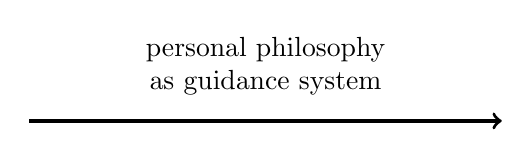
\begin{tikzpicture}[x=1cm,y=1cm]
\draw[->, very thick] (0,0) -- (6,0);
\node[align=center] at (3,0.7) {personal philosophy\\as guidance system};
\end{tikzpicture}
\caption{A cautious reconstruction of the first board idea: philosophy gives direction before it gives detail.}
\end{figure}

\subsection{Question \& Answer}

What does the guidance system actually do?

The lecture gives exactly two functions. We can write them in a compact schematic form as
\begin{equation}
G \longrightarrow \{\text{danger},\ \text{opportunity}\},
\end{equation}
where \(G\) denotes the guidance system.

The first function is negative in the best sense: it helps us see the dangers over here, so that we do not build on sand just because the sand presently looks attractive. The second function is positive: it helps us find the opportunities over there, so that we can move toward them deliberately rather than drift past them blindly.

What matters here is that the lecture does not treat danger and opportunity as separate subjects. A guidance system is necessary precisely because both are present at once. It must therefore begin early, with parents, teachers, ideas, and training, long before the consequences of bad judgment become irreversible.

\section{High Drama: Opposites, Temptation, and Conflict}

Once the guidance system is in place, the lecture widens into what Rohn calls ``high drama.'' The red-light example in Los Angeles is not comic filler. It is an explicit local model of the whole structure. The signal says one thing, the world may still contain another. The careless person does not have to be evil to be ruined; momentary thoughtlessness is enough.

The lecture then stacks examples: the childhood cartoon of angel and devil on opposite shoulders, the respected father who runs a light because he is late, the moral and business boundary one is tempted to cross, and the prayer that asks to be led around temptation rather than directly through it. The result is a general pattern rather than a collection of anecdotes.

A compact table captures the paired structure:
\begin{table}[h]
\centering
\begin{tabular}{p{0.34\linewidth} p{0.34\linewidth}}
danger & opportunity \\
evil & good \\
darkness & light \\
illness & health \\
death & life \\
tyranny & liberty
\end{tabular}
\caption{The lecture's paired opposites. The point is not symmetry for its own sake, but continual judgment between contrasted possibilities.}
\end{table}

Rohn compresses the whole section to one sentence worth preserving in displayed form:
\begin{equation}
\text{Opposites are in conflict and we are in the middle.}
\end{equation}

He then reinforces the point with biological metaphor: red corpuscles nourish, white corpuscles fight; friendly bacteria and unfriendly bacteria coexist; war is already running in the system. Even here the goal is not scientific exposition. The goal is structural clarity. Life is not a smooth text in which every chapter says that all is well. The drama exists because contest exists.

\subsection{Question \& Answer}

Why must danger and opportunity remain side by side?

The lecture's answer is that without the possibility of loss, the language of winning becomes empty. Without contest, a touchdown is not a touchdown. Without the pressure of alternatives, human drama disappears. We can say it in the stripped-down lecture form:
\begin{equation}
\text{no possibility of loss} \quad \Rightarrow \quad \text{no meaningful win}.
\end{equation}
Thus danger is not introduced to glorify danger. It is introduced to explain why judgment matters, why guidance is needed, and why the positive side must be actively chosen rather than passively assumed.

\section{Wind, Sail, and the Five-Year Redesign}

At exactly the point where ``high drama'' might become fatalistic, the lecture pivots back to agency. Philosophy becomes the set of the sail on a sailboat. Winds are always blowing: political winds, social winds, familiar winds, unfamiliar winds, and the violent upside-down winds of storm. The lecture's crucial move is to shift our attention from the uncontrollable term to the controllable one.

A compact editorial formula captures the logic:
\begin{equation}
\text{destination}=f(W,S),
\end{equation}
where \(W\) denotes the winds and \(S\) the set of the sail.

\begin{remark}
The lecture does not speak in this notation. What it explicitly says is that the wind is always blowing, and that one need not curse the wind if one learns to set a better sail.
\end{remark}

The same flip-chart page is reused across several minutes, and the broad layout survives even when the writing does not.

\begin{figure}[h]
\centering

\includegraphics[width=0.70\linewidth]{lecture_19_figure_03.png}
\caption{The accumulated flip-chart layout during the wind-and-storm discussion. What survives clearly is the structure: a central route, clustered regions, and a rising alternative path.}
\end{figure}

\begin{figure}[h]
\centering
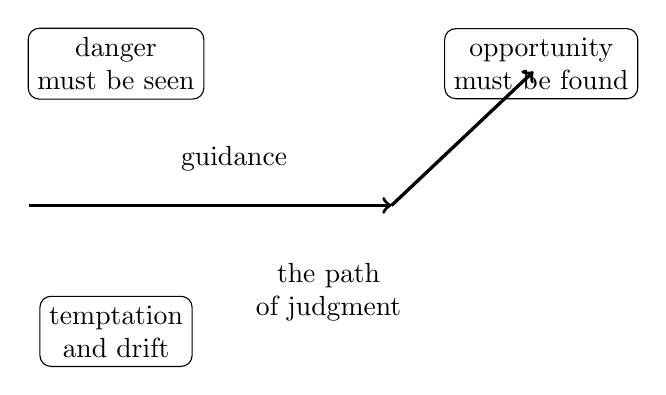
\begin{tikzpicture}[x=1cm,y=1cm]
\draw[->, very thick] (0.2,3.2) -- (4.8,3.2);
\draw[->, very thick] (4.8,3.2) -- (6.6,4.9);
\node[draw, rounded corners, align=center] at (1.3,5.0) {danger\\must be seen};
\node[draw, rounded corners, align=center] at (1.3,1.6) {temptation\\and drift};
\node[draw, rounded corners, align=center] at (6.7,5.0) {opportunity\\must be found};
\node[align=center] at (2.8,3.8) {guidance};
\node[align=center] at (4.0,2.1) {the path\\of judgment};
\end{tikzpicture}
\caption{A transcript-guided clarification of the board's logic: a central route, a dangerous side, and a rising opportunity side.}
\end{figure}

The sailboat analogy then becomes specifically human. A goose goes south because it is a goose. A human being can go north, south, east, or west by choice. A human being can also tear up a script lived for five years and write another one for the next five years. Here the lecture turns from metaphor to explicit redesign.

\subsection{Question \& Answer}

If the winds are given, what is actually ours to change?

The answer is: the set of the sail, the script we live by, the corrections we make in judgment, and the destination we are willing to name. The board's ``you are here'' moment is the local form of that answer.

\begin{figure}[h]
\centering

\includegraphics[width=0.70\linewidth]{lecture_19_figure_04.png}
\caption{Marking the current position on the five-year path sketch. The exact writing is uncertain, but the locator mark is the point.}
\end{figure}

We may summarize the redesign argument by distinguishing the present point \(x_0\), the destination reached by inertia, and the destination reached after correction:
\begin{align}
x_0 &\to x_{5,\mathrm{def}},\\
x_0 &\to x_{5,\mathrm{new}}.
\end{align}

\begin{figure}[h]
\centering
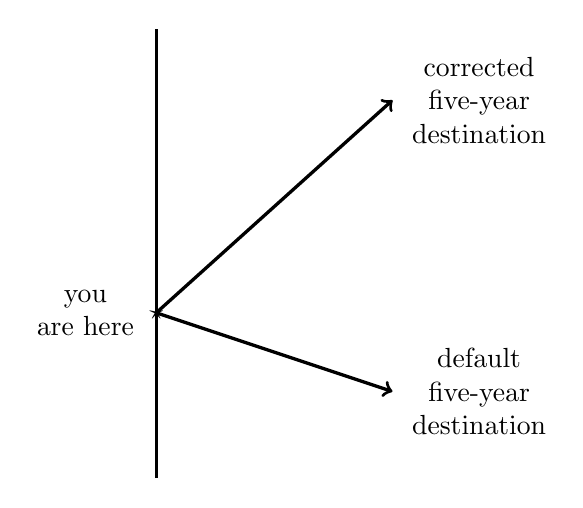
\begin{tikzpicture}[x=1cm,y=1cm]
\draw[very thick] (0,0) -- (0,5.7);
\draw[->, very thick] (0,2.1) -- (3.0,1.1);
\draw[->, very thick] (0,2.1) -- (3.0,4.8);
\node at (0,2.1) {$\star$};
\node[align=center] at (-0.9,2.1) {you\\are here};
\node[align=center] at (4.1,1.1) {default\\five-year\\destination};
\node[align=center] at (4.1,4.8) {corrected\\five-year\\destination};
\end{tikzpicture}
\caption{A narrow reconstruction of the redesign argument: continuation by inertia versus corrected direction.}
\end{figure}

\paragraph{Update rule.}
The logic of this redesign can be written as a worked sequence:
\begin{enumerate}
\item mark the present point \(x_0\);
\item extrapolate present daily activities to obtain \(x_{5,\mathrm{def}}\);
\item judge whether \(x_{5,\mathrm{def}}\) is acceptable;
\item identify errors in judgment and habits;
\item correct them and redirect motion;
\item arrive instead at \(x_{5,\mathrm{new}}\).
\end{enumerate}
This is precisely the argument Rohn attaches to his own age-\(25\) turning point: review the previous years, locate the errors, invest the corrections into the next years.

\section{Testimonials, Attitude, and Goal Formation}

After the redesign argument, the lecture pauses to stabilize the conclusion. Rohn does not say merely that redesign is logically conceivable. He says that testimonials and personal experience supply enough evidence to conclude that an extraordinary life can in fact be designed and lived. The mathematical spirit here is still present, but it is now evidentiary rather than arithmetic:
\begin{equation}
\text{testimonials}+\text{personal experience}
\Longrightarrow
\text{it is possible to design and live an extraordinary life}.
\end{equation}

This bridge matters because it prepares the move to attitude. Attitude is not introduced as a soft afterthought. It is introduced as the second major variable in the system: first what we know, then how we feel.

The lecture decomposes attitude into four directions. We need a good attitude toward the past, so that we use the past instead of carrying it as a burden. We need a good attitude toward the future, so that inspiration has a target. We need a good attitude toward everybody else, because enterprise and leadership require appreciation of the many and not merely the self. Finally we need a good attitude toward ourselves, because self-esteem generates self-confidence.

The future-directed part is made operational through goals. We decide what we want, write it down, make lists of people to meet, books to read, classes to take, skills to learn, cities to visit, and investments to acquire. Then we begin checking them off. The structure is elementary, but the lecture insists that it is powerful precisely because it is elementary.

\subsection{Question \& Answer}

How does inspiration become operational rather than merely emotional?

The answer is that inspiration must be tied to explicit lists, explicit check marks, and explicit celebration of completed items. A goal is not only a wish; it is a named future object that can later be checked off. In the lecture's sequence,
\begin{equation}
\text{self-esteem} \to \text{self-confidence} \to \text{larger action}.
\end{equation}

Rohn then enlarges the social meaning of attitude. One person does not make an economy, an orchestra, or an enterprise. It takes everybody. That is why appreciation of the gifts brought by others matters so much. The discussion of America as a depository of the world's gifts, the Rome anecdote, and the response to music all serve the same function: they teach us to value contribution, inheritance, and excellence outside ourselves.

\section{Activity, Labor, and the Rejection of Empty Affirmation}

The third great idea is activity. Here the lecture becomes causal again. Labor is not decorative. It is the mechanism by which nothing becomes something. Rohn states the old pattern in a form compact enough to write mathematically:
\begin{equation}
6\ \text{days labor} + 1\ \text{day rest}.
\end{equation}
In ratio form,
\begin{equation}
6:1.
\end{equation}

The lecture is careful here. It does not reject affirmation altogether. It rejects affirmation severed from truth and discipline. The truth-based example is intentionally hard-edged: if one is broke, the useful affirmation is not fantasy but truth. Only then can the truth act as a diagnostic signal.

\subsection{Question \& Answer}

Why is affirmation alone not enough?

Because affirmation does not perform the transformation. Labor performs the transformation. The lecture states the point in a line worth preserving as a displayed formula:
\begin{equation}
\text{affirmation without discipline} \to \text{delusion}.
\end{equation}

The deeper mechanism can be written in the paired form
\begin{align}
\text{wisdom}+\text{faith} &\not\Rightarrow \text{result} \qquad \text{without activity},\\
(\text{wisdom}+\text{faith}) \xrightarrow{\text{activity}} \text{result}.
\end{align}
Rohn's examples of the result are concrete: cities, careers, offices, health, relationships, fortunes. Even the lecture itself is included under this rule. It is work of language, work of words, work of phrasing ideas so that they may produce action elsewhere.

The phrase ``miracle working days'' is therefore not mystical escape from labor; it is praise of labor. These are miracle-working days precisely because work changes the state of the world.

\section{Measurement, Lifestyle, and the Closing Spiral}

The fourth idea is measure progress. Once work has been made central, the next danger is self-deception. One may feel that things are fine when they are not fine. Thus the lecture adds a counting discipline:
\begin{equation}
\text{progress}=\text{measurable in reasonable time}.
\end{equation}

The lecture defines reasonableness by contrast. Five minutes is too soon; nothing has happened yet. Five years is too late; too much can have gone wrong. The daily check therefore becomes the basic cadence.

\begin{table}[h]
\centering
\begin{tabular}{p{0.28\linewidth} p{0.46\linewidth}}
too soon & every five minutes \\
reasonable & by the end of the day \\
too late & after five years of not looking
\end{tabular}
\caption{The lecture's measurement cadence.}
\end{table}

The child-level example is especially clear:
\begin{equation}
1\ \text{grade} / 1\ \text{year}.
\end{equation}
This is not because all human development is scholastic. It is because the example makes progress countable. The same logic applies to property counts, income counts, health checks, and the building of a financial wall around one's family.

\subsection{Question \& Answer}

Why must we measure when things may already look fine from the outside?

Because appearance is not the same as structure. The vineyard may look good while little foxes are already working at the vines. A full bank account may be one sign, but it may not be the decisive sign. Thus the lecture's practical theorem is simple:
\begin{equation}
\text{success is a numbers game}.
\end{equation}
Count, check, and do not wait for society or government to build the measuring system for you.

From here the talk widens once more. Rohn recaps the five ideas, briefly stages the long debate with Zig Ziglar about education and motivation, and then adds the fifth theme, lifestyle. The essence of life, he says, is not reducible to the Ferrari or the bank account. A good life contains productivity, enduring friendship, living heritage, spirituality studied and practiced and taught, and a refusal to miss the richness of experience.

Even in this widening close, the lecture remains structurally consistent. The good life is not passive consumption. It is productive participation. It is appreciation of extraordinary value wherever it appears: music, poetry, conversation, friendship, and the cultivated quality of things. The wine anecdote belongs here not as luxury for its own sake, but as an example of recognition. Something in us is supposed to notice excellence.

The final theological image is entirely continuous with the rest of the chapter. If we plant the seed, the tree is not ours to manufacture directly. But we are invited to participate in the working of miracles. Work of hands, work of language, work of the caring soul: the lecture ends by treating these not as separate from success, but as its highest form.

\section{Summary}

This chapter begins with a ladder and ends with a life. The ladder tells us that large increases in earning are possible. The lecture then explains the operative variable: value to the marketplace, developed by working harder on ourselves than on our job. Personal philosophy is introduced as a guidance system, then widened into a drama of opposed possibilities, and then returned to human agency through the sailboat and the five-year redesign. Attitude gives this redesign motive force, activity gives it causal power, measurement gives it discipline, and lifestyle gives it human meaning. The closing claim is therefore broader than ambition alone: we are not only trying to earn more, but to live deliberately enough to participate in the making of something larger than ourselves.